% ch1.tex
% Dieses Werk ist unter einem Creative Commons Namensnennung-Keine kommerzielle Nutzung-Weitergabe 
% unter gleichen Bedingungen 3.0 Deutschland Lizenzvertrag lizenziert. Um die Lizenz anzusehen, gehen Sie bitte 
% zu http://creativecommons.org/licenses/by-nc-sa/3.0/de/ oder schicken Sie einen Brief an 
% Creative Commons, 171 Second Street, Suite 300, San Francisco, California 94105, USA.


\chapter{Not all snakes will squish you}\label{ch:notallsnakeswillsquishyou}

Chances are you were given this book for your birthday.  Or possibly for Christmas.  Aunty Mildred was going to give you mismatching socks that were two sizes too large (and you wouldn't want to wear when you grew into them anyway).  Instead, she heard someone talking about this printable book, remembered you had one of those computer-thingamabobs that you tried to show her how to use last Christmas (you gave up when she started trying to talk into the mouse), and got them to print another copy.  Just be thankful you didn't get the mouldy old socks.

I hope you're not too disappointed that I popped out of the recycled wrapping paper, instead.  A not-quite-so-talkative (okay, not-talking-at-all) book, with an ominous looking title on the front about ``Learning$\ldots$''.
But take a moment to think about how I feel.  If you were the character from that novel about wizards that is sitting on the bookshelf in your bedroom, I'd possibly have teeth... or perhaps even eyes.  I might have moving pictures inside me, or be able to make moaning ghostly sounds when you opened my pages.  Instead, I'm printed out on dog-eared A4 sheets of paper, stapled together or perhaps bound in a folder.  How would I know---I don't have eyes.
\\
\\
\emph{I'd give anything for a nice, sharp set of teeth$\ldots$}
\\
\\
However it's not as bad as it sounds.  Even if I can't talk... or bite your fingers when you're not looking... I can tell you a little bit about what makes computers work.  Not the physical stuff, with wires and computer-chips and cables and devices that would, more than likely, electrocute you as soon as you touched them (so don't!!)---but the hidden stuff running around inside those wires and computer-chips and cables and bits, which make computers actually useful.

\begin{wrapfigure}{r}{0.5\textwidth}
  \begin{center}
\includegraphics*[width=70mm]{electrocute.eps}
  \end{center}
\end{wrapfigure}

It's a little like thoughts running around inside your head. If you didn't have thoughts you'd be sitting on the floor of your bedroom, staring vacantly at the door and drooling down the front of your t-shirt. Without \emph{programs}, computers would only be useful as a doorstop---and even then they wouldn't be very useful, because you'd keep tripping over them in the night.  And there's nothing worse than a stubbed toe in the dark.
\\
\\
\emph{I'm just a book and even I know that.}
\\
\\
Your family may have a Playstation, Xbox or Wii sitting in the lounge---they're not much use without programs (Games) to make them work.  Your DVD player, possibly your fridge and even your car, all have computer programs to make them more helpful than they would be otherwise.  Your DVD player has programs to help it figure out what to play on a DVD; your fridge might have a simple program to make sure it doesn't use too much electricity, but still keep your food cold; your car might have a computer with a program to warn the driver if they're about to bump into something.\\
If you know how to write computer programs, you can do all sorts of useful things. Perhaps write your own games. Create web pages that actually do stuff, instead of just sitting there looking somewhat colourful.  Being able to program could possibly even help with your homework.\\
\\
That said, let's get onto something a bit more interesting.

\section{A Few Words About Language}

Just like humans, certainly whales, possibly dolphins, and maybe even parents (although that's debatable), computers have their own language.  Actually, also like humans, they have more than one language.  There are languages covering just about all the letters of the alphabet.  A, B, C, D and E are not only letters, they're also programming languages (which proves that adults have no imagination, and should be made to read either a dictionary or a thesaurus before naming anything).

There are programming languages named after people, named using simple acronyms (the capital letters of a series of words), and just a few named after a TV show.  Oh, and if you add a few pluses and hashes (+, \#) after a couple of those letters I just listed---that's yet another couple of programming languages as well.  Making matters worse, some of the languages are almost the same, and differ only slightly.
\\
\\
\emph{What did I tell you?  No imagination!}
\\
\\
Luckily, many of these languages have fallen into disuse, or vanished completely; but the list of different ways you can `talk' to a computer is still rather worryingly large.  I'm only going to discuss one of them---otherwise we might as well not even get started.
\\
It would be more productive to sit in your bedroom and drool down the front of your t-shirt$\ldots$

\section{The Order of Non-venomous\\Constricting Serpentes$\ldots$}

$\ldots$or Pythons, for short.

Apart from being a snake, Python\index{Python} is also a programming language.  However, it was not named after a legless reptile; rather it is one of the few programming languages named after a TV show.  Monty Python was a British comedy show popular during the 1970's (and still popular now, actually), which you have to be a certain age to find amusing.  Anyone below the age of about$\ldots$ let's say 12$\ldots$ will wonder what all the fuss is all about\footnote{Except the fish slapping dance.  That's funny no matter how old you are.}.

There are a number of things about Python (the programming language, not the snake, nor the TV show) that make it extremely useful when you're learning to program.  For us, at the moment, the most important reason is that you can start it up and do stuff really quickly.

This is the part where you hope Mum, Dad (or whomever is in charge of the computer), has read the part at the beginning of this book labelled ``A Note for Mums and Dads''.

\noindent
There's a good way to find out if they actually have read it:

\begin{WINDOWS}
Click on the Start button at the bottom left of the screen, click on `All Programs' (which has a green triangle next to it), and hopefully in the list of programs you should see `Python 2.5' (or something like it).  Figure~\ref{fig1} shows you what you should be looking for. Click on `Python (command line)' and you should see something like Figure~\ref{fig2}.

\begin{figure}
\begin{center}
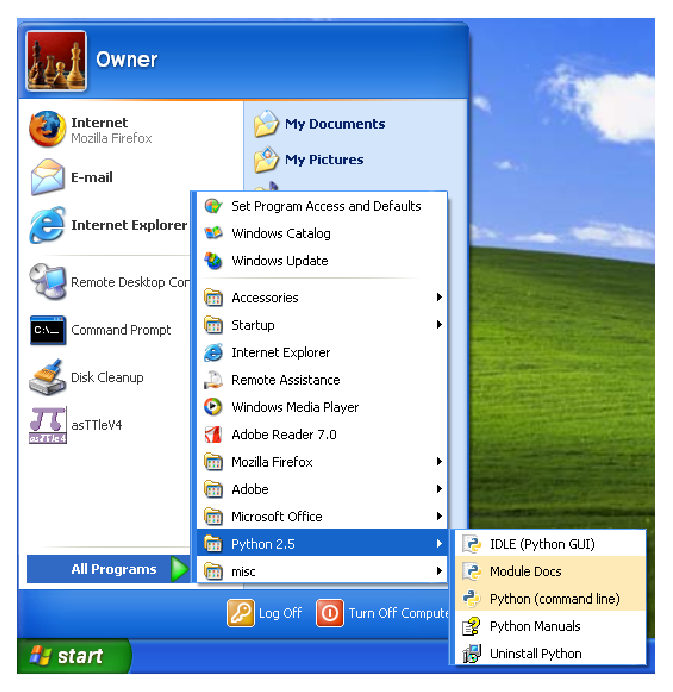
\includegraphics[width=80mm]{figure1.eps}
\end{center}
\caption{Python in the Windows menu.}\label{fig1}
\end{figure}

\begin{figure}
\begin{center}
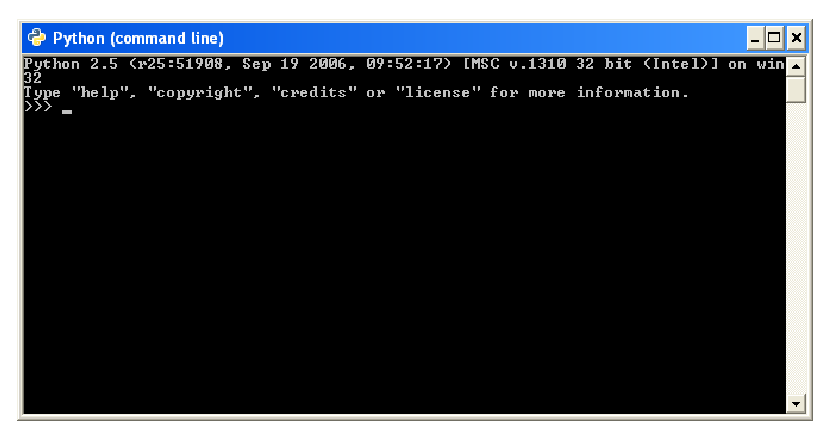
\includegraphics[width=135mm]{figure2.eps}
\end{center}
\caption{The Python console on Windows.}\label{fig2}
\end{figure}
\end{WINDOWS}

\begin{MAC}
In Finder, on the left you should see a group called `Applications'.  Click on this, and then find a program called `Terminal' (it'll probably be in a folder called `Utilities').
Click on `Terminal', and when it starts up, type python and hit enter.  You'll should hopefully be looking at a window that looks like Figure~\ref{fig3}.

\begin{figure}
\begin{center}
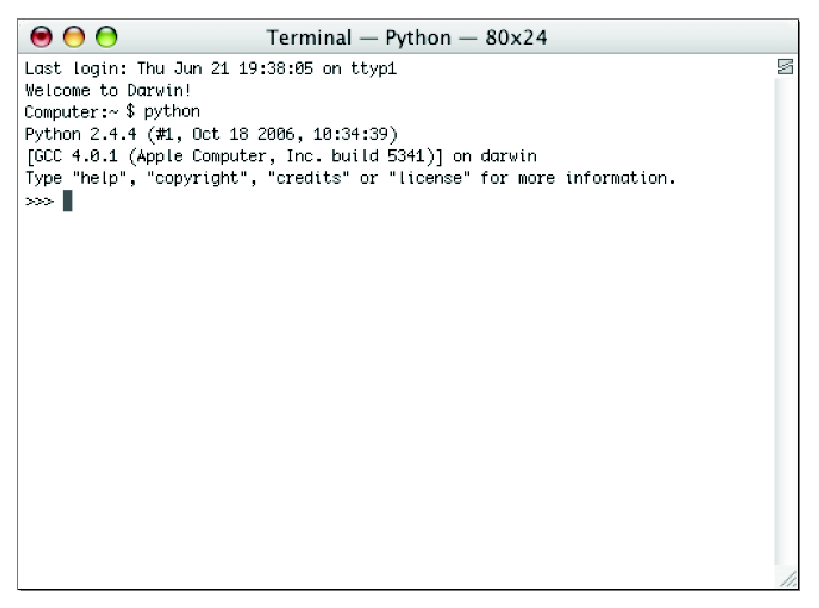
\includegraphics[width=85mm]{figure3.eps}
\end{center}
\caption{The Python console on Mac OSX.}\label{fig3}
\end{figure}
\end{MAC}

\begin{LINUX}
Ask Mum or Dad which terminal application you should use (it could be one called `Konsole', `rxvt', `xterm' or any one of a dozen different programs---which is why you'll probably need to ask).  Start the terminal program and type `python' (without the quotes), and hit enter.  You should see something like Figure~\ref{fig4}.

\begin{figure}
\begin{center}
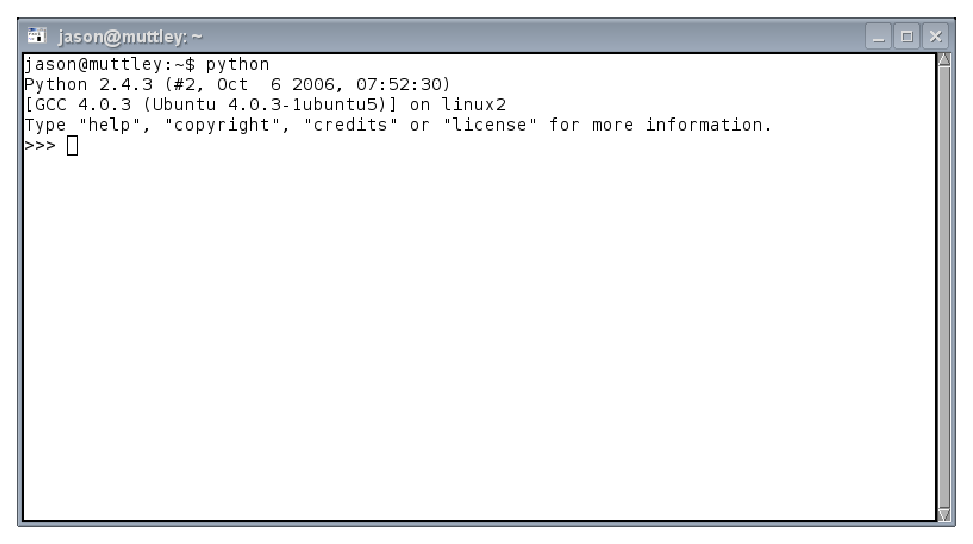
\includegraphics[width=80mm]{figure4.eps}
\end{center}
\caption{The Python console on Linux.}\label{fig4}
\end{figure}
\end{LINUX}

\subsection*{\color{BrickRed}If you discover they haven't read the section in the beginning$\ldots$}

$\ldots$because there is something missing when you try to follow those instructions---then turn to the front of the book, poke it under their nose while they're trying to read the newspaper, and look hopeful.  Saying, ``please please please please'' over and over again, until it becomes annoying, might work quite well, if you're having trouble convincing them to get off the couch.  Of course, the other thing you can do, is turn to the front of the book, and follow the instructions in the Preface to install Python yourself.

\section{Your first Python program}

With any luck, if you've reached this point, you've managed to start up the Python console, which is one way of running Python commands and programs.  When you first start the console (or after entering a command), you'll see what's called a `prompt'.  In the Python console\index{Python console}, the prompt is three chevrons, or greater-than symbols ($>$) pointing to the right:

\begin{listing}
\begin{verbatim}
>>>
\end{verbatim}
\end{listing}

If you put enough Python commands together, you have a program that you can run in more than just the console$\ldots$ but for the moment we're going to keep things simple, and type our commands directly in the console, at the prompt ($>>>$).  So, why not start with typing the following:

\begin{listing}
\begin{verbatim}
print("Hello World")
\end{verbatim}
\end{listing}

Make sure you include the quotes (that's these: $"$ $"$), and hit enter at the end of the line.  Hopefully you'll see something like the following:

\begin{listing}
\begin{verbatim}
>>> print("Hello World")
Hello World
\end{verbatim}
\end{listing}

The prompt reappears, to let you know that the Python console is ready to accept more commands.

\noindent
Congratulations! You've just created your first Python program.  \code{print} is a function that writes whatever is inside the brackets out to the console--we'll use it more later.

\section{Your Second Python program$\ldots$the same again?}

Python programs wouldn't be all that useful if you had to type the commands every single time you wanted to do something---or if you wrote a program for someone, and they had to type it in before they could use it.

The Word Processor that you might be using to write your school assignments, is probably somewhere between 10 and 100 million lines of code.  Depending upon how many lines you printed on one page (and whether or not you printed on both sides of the paper), this could be around 400,000 printed pages$\ldots$ or a stack of paper about 40 metres high.
Just imagine when you brought that software home from the shop, there would be quite a few trips back and forth to the car, to carry that much paper$\ldots$

$\ldots$and you'd better hope there's no big gust of wind while you're carrying those stacks. Luckily, there's an alternative to all this typing---or no one would get anything done.

\begin{center}
\includegraphics*[width=85mm]{pullinghair.eps}
\end{center}

\begin{WINDOWS}
Open Notepad (Click on Start, All Programs, and it should be in the Accessories sub menu), and then type the print command exactly as you typed it into the console before:

\begin{listing}
\begin{verbatim}
print("Hello World")
\end{verbatim}
\end{listing}

Click on the File menu (in Notepad), then Save, and when prompted for a file name, call it \emph{hello.py} and save it on your Desktop. Double-click on the icon for hello.py on your Desktop (see Figure~\ref{fig5}) and for a brief moment a console window will appear.  It will vanish too quickly for you too make out the words, but Hello World will have been printed to the screen for a fraction of a second---we'll come back to this later and prove that it did.\\

\begin{figure}
\begin{center}

\includegraphics[width=58mm]{figure5.eps}
\end{center}
\caption{hello.py icon on the Windows Desktop.}\label{fig5}
\end{figure}
\end{WINDOWS}

\begin{MAC}
Open up the Text Editor by clicking on its icon.  It may be in the Dock at the bottom of the screen \includegraphics*[width=12mm]{textedit-icon.eps}, or look for this icon \includegraphics*[width=19mm]{textedit-icon2.eps} in the Applications list in Finder.  Type the print command exactly as you typed it into the console earlier:

\begin{listing}
\begin{verbatim}
print("Hello World")
\end{verbatim}
\end{listing}

Click on the File menu, then click on Save, and when you are prompted for a file name, call it hello.py and save it into your home directory (your home directory is on the left under Places--ask Mum or Dad to point it out for you).

Open the `Terminal' application again--it will automatically start up in your home directory--and type the following:

\begin{listing}
\begin{verbatim}
python hello.py
\end{verbatim}
\end{listing}

You should see Hello World written to the window exactly as it was when you typed the command in the Python console.

\end{MAC}

\begin{LINUX}
Open a text editor (again you might have to ask Mum or Dad which one to use), then type the print command exactly as you typed it into the console:

\begin{listing}
\begin{verbatim}
print("Hello World")
\end{verbatim}
\end{listing}

Click on the File menu, then Save, and when prompted for a file name, call it hello.py and save it in your Home folder (there might be an icon called `Home' somewhere in the Save dialog box).  Next open up the terminal application (again Konsole, rxvt, etc... what we used earlier), and type:

\begin{listing}
\begin{verbatim}
python hello.py
\end{verbatim}
\end{listing}

You should see Hello World written to the window exactly as it was when you typed the command in the Python console (see Figure~\ref{fig9}).

\begin{figure}
\begin{center}
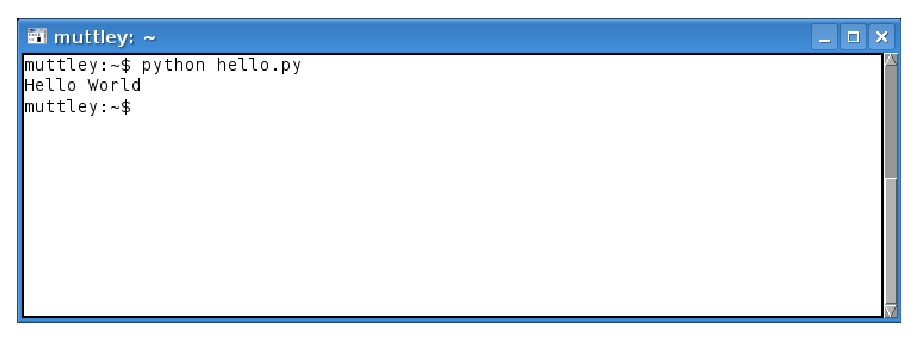
\includegraphics[width=75mm]{figure9.eps}
\end{center}
\caption{Running a python program from a text file on Linux.}\label{fig9}
\end{figure}
\end{LINUX}

So you can now see that the nice people who created Python, have kindly saved you from having to type the same thing over and over and over and over and over again.  Like they did back in the 1980's.  No, I'm serious---they did.  Go and ask your Dad if he ever owned a ZX81 when he was younger?\\

\noindent
If he did you can point at him and laugh.\\

\noindent
Trust me on this one.  You won't get it.  But he will.\footnote{The Sinclair ZX81, released in the 1980's was one of the first affordable home computers.  A number of young boys and girls were driven completely mad, typing in the code for games printed in popular ZX81 magazines---only to discover, after hours of typing, that the darn things never worked properly.}

\noindent
\emph{Be prepared to run away though.}

\subsection*{\color{BrickRed}The End of the Beginning}

Welcome to the wonderful world of Programming.  We've started really simply with a ``Hello World'' application---everyone starts with that, when they're learning to program.
In the next chapter we'll start to do some more useful things with the Python console and then look at what goes into making a program.

\newpage
